%4. Problem space (Prototype, test setups, existing software)
\chapter{Understanding the Problem Space}
\label{chap:understanding-the-problem-space}
In order to provide a satisfying solution to the problem at hand, the problem itself and the environment it occurs in must be researched. This chapter aims to explore and examine the problem space, resulting in a set of artefacts (namely a domain model and a set of requirements) that aid in understanding the context and designing an appropriate solution. First, a prototypical network proxy is designed and implemented in section \ref{sec:prototypical-implementation} to get an understanding of the problems and challenges involved in designing, implementing and using such software. Based on these experiences, interviews with experts in penetration testing are conducted and evaluated in section \ref{sec:interviews} to get a proper understanding of their everyday work and resulting problems. Lastly, existing software that aims to intercept communication for various scenarios and technologies is examined in section \ref{sec:analysis-existing-software}, compared to each other and their usefulness for the problem-specific scenarios is assessed.

\section{Prototypical Implementation}
\label{sec:prototypical-implementation}
The prototype was designed to be used in three different scenarios, each taking place in a different context. The goal of this section was to implement a prototype that could be used as a proxy to intercept communication between an \ac{IoT} device and its cloud service as shown in figure \ref{fig:network-communication-diagrams}. It was developed incrementally so individual components could be derived from requirements, designed, implemented and evaluated in fixed sprints.

\begin{figure}%
    \centering
    \subfloat[\centering Regular communication between an \ac{IoT} device and a cloud service.]{{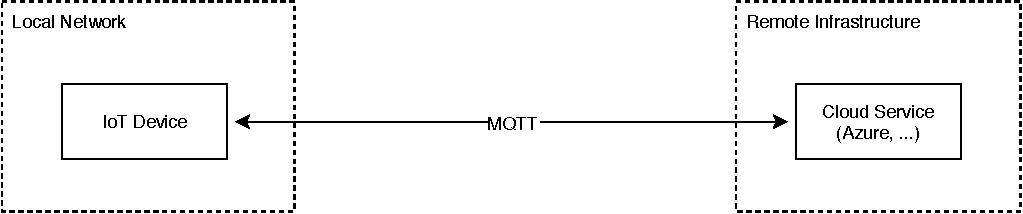
\includegraphics[width=10cm]{img/ch04/Setup - 1 Regular.pdf} }}%
    \qquad
    \subfloat[\centering Communication intercepted by a \ac{MITM} proxy.]{{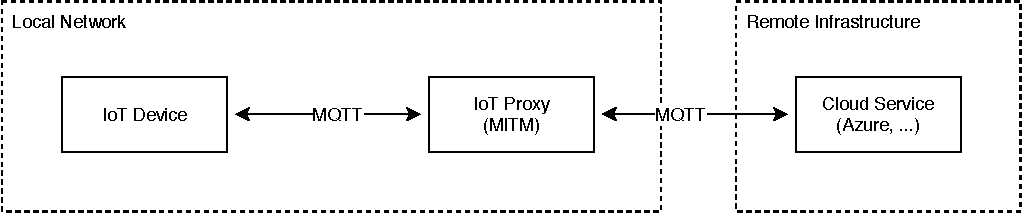
\includegraphics[width=10cm]{img/ch04/Setup - 2 Pentesting.pdf} }}%
    \caption{Installing a \ac{MITM} proxy to intercept network communication for penetration testing.}%
    \label{fig:network-communication-diagrams}%
\end{figure}

\subsection{Example Scenarios}
\label{sec:example-scenarios}
The following scenarios describe hypothetical configurations of \ac{IoT}/\ac{IIoT} devices that should be tested with the prototype and vary in both technical and logical complexity as well as in closeness to reality:

\paragraph{Scenario \#1: Legacy \ac{ICS} Application}
In this \ac{IIoT} scenario, a \ac{HMI} (\emph{Siemens KTP400 Basic}) sends commands to and receives data from a \ac{PLC} (\emph{Siemens S7-1200}) using Modbus \ac{TCP}. The \ac{PLC} continually counts up a value up to 100 and begins anew at zero while the \ac{HMI} displays the current value and provides a button that, upon being pressed by a user, resets the current value to zero. \\
In this scenario, attackers could perform a variety of attacks on the system by intercepting and manipulating network traffic, for example:
\begin{itemize}
    \item By dropping messages sent from the \ac{PLC} to the \ac{HMI}, the application may appear unresponsive as new data is not displayed on the \ac{HMI}. In production environments, this could lead to dangerous situations as sensor readings that indicate harmful environmental conditions would not be presented to supervising personnel.
    \item When dropping messages sent from the \ac{HMI} to the \ac{PLC}, control commands can be suppressed. This attack can result in catastrophic situations when emergency shutdowns issued by supervising personnel are not registered by the affected machines.
\end{itemize}
This scenario is of an academic nature and does not depict a realistic \ac{ICS} process, but focusses on the use of a legacy transport protocol. Due to the rather simple nature of the Modbus \ac{TCP} protocol, intercepting and manipulating communication is expected to be trivial. %TODO: Add diagram?
%https://support.industry.siemens.com/tf//WW/en/posts/s7-1500-communication-and-modbus-tcp-on-hmi/144092?page=0&pageSize=10
%https://support.industry.siemens.com/cs/pd/379924?pdti=td&dl=en&lc=en-DK

\paragraph{Scenario \#2: \ac{IoT} Cloud Application} This \ac{IoT} smart home scenario utilizes two local \ac{IoT} devices that are integrated into a cloud environment such as the \ac{AWS} \ac{IoT} platform: a thermometer and an \ac{A/C} unit. Both devices connect to the cloud platform, authorize themselves at a \ac{REST} interface via \ac{HTTP} and upgrade their \ac{HTTP}-connection to \ac{WS} streams upon successful authorization. They eventually communicate to a remote \ac{MQTT} broker by tunnelling \ac{MQTT} packets over the \ac{WS} stream. At this stage, the thermometer publishes temperature readings to an \ac{MQTT} topic while the \ac{A/C} unit subscribes to the same topic and adjusts its operation depending on the incoming temperature readings. \\
This distributed communication setup introduces a set of possible attacks that could be performed when attackers \emph{impersonated} client-devices or the remote server:
\begin{itemize}
    \item Impersonating the thermometer, attackers could send incorrect temperature data and effectively control the \ac{A/C} unit. When sending low temperature readings while the environment temperature is high, the \ac{A/C} unit would stop running. Conversely, when high temperature readings are sent while the environment temperature is low, the \ac{A/C} unit would run, and thus further cool down the environment.
    \item Attackers that impersonate the remote server could drop or manipulate incoming publish packets, thus altering whether and/or what information is relayed other connected devices. For example, temperature readings that indicate a high environment temperature that would lead to the \ac{A/C} unit to be powered up could be rewritten in such a way that the transmitted temperature value is considered to indicate a low environment temperature, thus preventing the \ac{A/C} unit from running automatically.
\end{itemize}

\begin{figure}[ht]
    \centering
    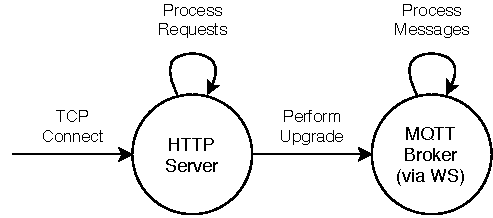
\includegraphics[width=6cm]{img/ch04/Statemachine 2.pdf}
    \captionof{figure}{State machine of \ac{AWS} \ac{IoT} communication}
    \label{fig:aws-statemachine}
\end{figure}
This scenario makes use of three communication protocols, uses these protocols dependent on the state of authentication and even tunnels one protocol through another one. Therefore the proxy application has to implement a state-machine (as seen in figure \ref{fig:aws-statemachine}) and testing communication in this scenario is expected to be more complex than the first one. Also, since this scenario makes use of the \ac{AWS} \ac{IoT} infrastructure, special care must be taken to ensure that authentication is properly relayed to the cloud servers.

% Reference: https://aws.amazon.com/blogs/aws/aws-iot-cloud-services-for-connected-devices/

\paragraph{Scenario \#3: Water Treatment Plant} Similar to scenario \#2, this scenario makes use of \ac{MQTT} for transporting messages. However, the scenario takes place in an \ac{ICS} context of critical infrastructure.

\begin{figure}[hb]
    \centering
    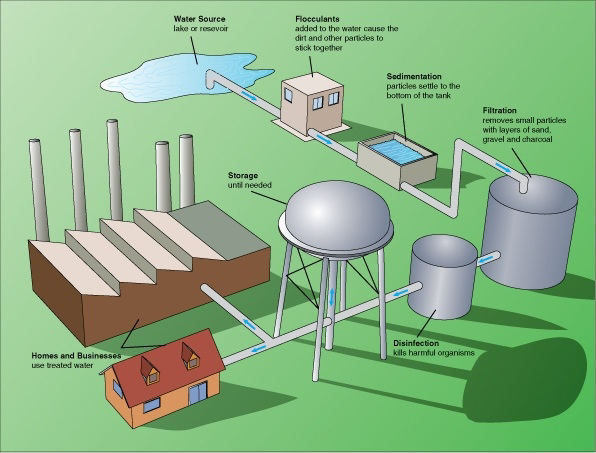
\includegraphics[width=12cm]{img/ch04/watertreatmentplant.png}
    \captionof{figure}{\enquote{Illustration of a typical drinking water treatment process.} (by the CK-12 Foundation)} %\footnote{https://en.wikipedia.org/wiki/File:Illustration\_of\_a\_typical\_drinking\_water\_treatment\_process.png}
    \label{fig:water-treatment}
\end{figure}

As shown in figure \ref{fig:water-treatment}, there are multiple steps involved in treating water for drinking. The scenario represents these steps as separate stations (\enquote{source}, \enquote{flocculants}, \enquote{sedimentation}, \enquote{filtration} and \enquote{storage}) that act as \ac{MQTT} clients. Each station receives water into an input tank, processes water from its input tank in a specified rate and flushes processed water into an output tank. Similar to how threads can suffer from starvation in a multithreading environment, these stations can either \enquote{run dry} when their input tank is empty or overflow when either tank is filled beyond their capacity. In this scenario, stations will only process water from their input tanks if their output tank provides sufficient available capacity.\\
Similar to scenario \#2, attackers could perform a series of attacks in this scenario:
\begin{itemize}
    \item Without intercepting any communication, attackers could cyclically overwrite water levels of either input and output tanks to stop stations and bring processing to a halt. For example, when attackers overwrite the \enquote{storage} station's input tank level to indicate exhausted capacities, the \enquote{disinfection} station would fill its output tank and eventually stop processing water. This would cause the \enquote{disinfection} station's input tank to fill up and lead to the \enquote{filtration} station's output tank to fill up. Ultimately, the water treatment plant would halt.
    \item When any station publishes data about its tanks' levels indicating full or empty capacities, attackers could intercept those messages and change them to either indicate the opposite (change tank levels indicating \emph{full} capacities to levels indicating \emph{empty} capacity) or some arbitrary level information. This could lead to either pumping water from empty tanks, potentially damaging the pumps, or to overfilling tanks, leading to leaking excess water and potentially damaging further equipment.
\end{itemize}
This scenario greatly simplifies drinking water treatment by reducing the process to the producer-consumer problem known from multithreading. A more realistic representation of drinking water treatment plants would take further details, such as chemicals used in disinfection, into account.\\
This scenario involves only \ac{MQTT} as a transport protocol but requires six \ac{MQTT} clients to run simultaneously.


\subsection{Requirements}
To be able to operate in all of the aforementioned scenarios, the prototype had to implement a set of functional requirements:
\begin{itemize}
    \item [\textbf{F1}] \textbf{Protocols:} The software must implement parsing/crafting messages/packets of the following communication protocols: \ac{HTTP}, \ac{WS}, \ac{MQTT} and Modbus \ac{TCP}. \\
          \textit{Fit criterion: The software must implement and support the \ac{HTTP}, \ac{WS} and \ac{MQTT} protocols so messages of those protocols can be further processed by the software.}
    \item [\textbf{F2}] \textbf{Network Stacks:} The software must be able to parse protocols that are tunnelled through other protocols (\enquote{\emph{stacked}}). It must provide an interface to the user where they can specify which communication protocols are used and whether and how they are stacked (further referred to as \emph{network stack}).\\
          \textit{Fit criterion: The software processes a configuration file that lets users specify which protocols to be used and whether/how they are stacked.}
    \item [\textbf{F3}] \textbf{State-Machines:} The software must be able to switch network stacks and scripts for processing dependent on configurable \emph{states} and \emph{transitions} between them. It must provide an interface for the user to specify when to switch to using another network stack, represented using \acp{FSM} and rule sets for transmission between states.\\
          \textit{Fit criterion: The software processes a configuration file that lets users specify when to switch between network stacks.}
    \item [\textbf{F4}] \textbf{Integration:} The software shall provide interfaces for integration of third-party software.\\
          \textit{Fit criterion: The software implements interfaces that allow sending packets to other applications such as \enquote{Burp Suite}.}
    \item [\textbf{F5}] \textbf{Scripting:} The software shall provide scripting capabilities for automated manipulation of messages/packets.\\
          \textit{Fit criterion: Users can define script-snippets to be executed on messages/packets.}
\end{itemize}

The following non-functional requirements were defined:

\begin{itemize}
    \item [\textbf{N1}] \textbf{Extensibility:} To allow for future implementation of further communication protocols the software shall be implemented in a modular fashion.
    \item [\textbf{N2}] \textbf{Platform Compatibility:} In order to support a broad spectrum of target platforms, the software shall be implemented platform-independently.
    \item [\textbf{N3}] \textbf{Reusability:} The software shall be reusable so it can be used in future tests that may feature new configurations of network stacks.
    \item [\textbf{N4}] \textbf{Open Source:} The software shall be available as open source software so programmers and members of the IT community may contribute to improving it.
\end{itemize}

Due to this implementation serving as a prototype and being of an academic nature, no specific constraints were defined. It was to be developed strictly ignoring aspects of usability and stability as it should not be used in production environments but in laboratories exclusively.

\subsection{Design}
The prototype was designed to be fit for use in the second scenario as, regarding network communication, it was more complex than the other ones. Specifically, the second scenario demanded the implementation of a network stack and a state machine to switch between states.
Parsing protocols that were tunnelled through other protocols appeared to be a potentially challenging requirement. In order to tackle it, a variation of the \emph{\enquote{pipeline}} (sometimes referred to \emph{\enquote{pipes and filters}}) design pattern was used (as shown in figure \ref{fig:design-pipes-and-filters}). It was designed to be used as follows:\par
\enquote{Messages} originate from a listener, for example messages with raw byte payloads are received from a \ac{TCP} socket. These messages are sent to an initial \enquote{pipe} to be processed \emph{down}.
Pipes are bi-directional routers that perform the following actions on messages:
\begin{enumerate}
    \item Use optional \enquote{encoders} to disassemble/de-serialize messages when processing them \emph{down} the pipeline and re-assemble/serialize them when they process messages \emph{up} the pipeline.
    \item Use optional \enquote{filters} to perform operations on messages such as replacing header values or manipulating payloads.
    \item Forward messages to the next pipe in its pipeline when processing messages down or to the previous pipe when processing messages back up.
\end{enumerate}
There are extensions to basic pipes such as:
\begin{itemize}
    \item \enquote{EndPipes} are appended to the end of a pipeline and reverse the message processing direction so messages that were processed down are sent back up the pipeline to be processed up.
    \item \enquote{ProcessingPipes} mandate encoders and filters to be used. These pipes are used to indicate that messages are not not only routed but also processed and encoded or decoded.
    \item \enquote{IntegrationPipes} allow integration of other software into the pipeline. For example, penetration testing software such as Burp Suite could be integrated.
\end{itemize}

\emph{TBD:}
\begin{itemize}
    \item \emph{Designed during sprints so only pipes are designed, state-machine only rough concept (States, Transitions, Rules)!}
    \item \emph{Show diagrams of messages?}
    \item \emph{Explain Figure \ref{fig:app-diag-pipesfilters-1} and \ref{fig:app-diag-pipesfilters-2}}
\end{itemize}


\begin{figure}
    \centering
    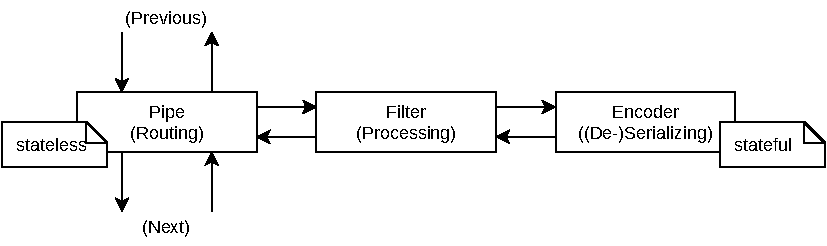
\includegraphics[width=14cm]{img/ch04/Architecture - Pipes and Filters3.pdf}
    \captionof{figure}{The variation of the \emph{\enquote{pipes and filters}}/\emph{\enquote{pipeline}} design pattern used in the prototype.}
    \label{fig:design-pipes-and-filters}
\end{figure}

\subsection{Testing}
\label{sec:prototype-testing}
To test the prototype, a simple testbed was designed and implemented to realize scenario \#3 (discussed in section \ref{sec:example-scenarios}). It consisted of two Debian 10 machines that acted as a \ac{MQTT} broker and clients and a Kali Linux machine that ran the prototype and provided tools such as Wireshark that could be used for debugging and monitoring network traffic. All machines were connected to a single network (shown in figure \ref{fig:testbed}) and were assigned static \ac{IP} addresses. While this setup allowed for more sophisticated \ac{MITM} mechanisms such as \ac{ARP} spoofing, the decision was made to directly connect the \ac{MQTT} clients to the \emph{kali} machine to reduce complexity and accelerate and simplify testing. Separate machines were used for the \ac{MQTT} broker and clients so that actual \ac{MITM} attacks could be performed if the need to arose. Also, running the broker on a separate machine simplified debugging as network traffic could be attributed to broker or clients easier by examining the packets' source and destination \acp{IP}.\par

\begin{figure}[h]
    \centering
    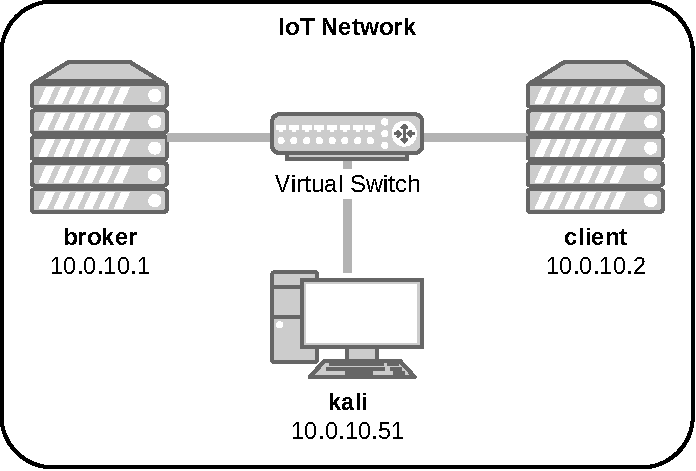
\includegraphics[width=8cm]{img/ch04/Testbed2.pdf}
    \captionof{figure}{A network diagram of the testbed that was used for testing the prototype.}
    \label{fig:testbed-network}
\end{figure}
The \ac{MQTT} broker software used on the \emph{broker} machine was Eclipse Mosquitto\footnote{https://mosquitto.org/} $1.5.7$ and had the \ac{WS} transport enabled to allow for clients to connect via \ac{WS}. The \ac{MQTT} clients running on the \emph{client} machine were implemented in Python using the Eclipse Paho library for Python (paho-mqtt\footnote{https://pypi.org/project/paho-mqtt/}).\par %TODO: Describe publish and processing pattern, ref mqtt graph below
\begin{figure}[h]
    \centering
    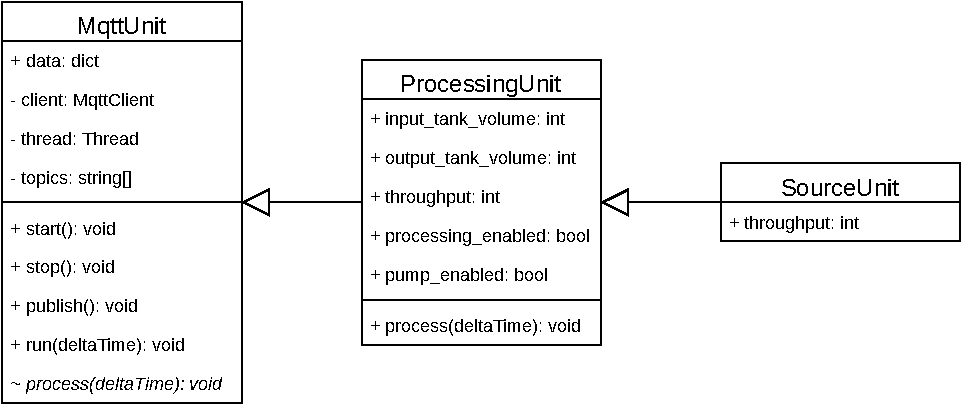
\includegraphics[width=14cm]{img/ch04/Testbed-Unit.pdf}
    \captionof{figure}{The \enquote{ProcessingUnit} data-structures represent individual stations of the simplified water treatment plant.} %TODO: Describe
    \label{fig:testbed-unit}
\end{figure}
The water treatment scenario required water treatment stations to be simulated individually as separate \ac{MQTT}, which was done by representing them as \enquote{ProcessingUnits} in the Python implementation of the testbed. As can be seen in figure \ref{fig:testbed-unit}, ProcessingUnits held individual \emph{MqttClient} instances running in separate threads, were subscribed to the topics of relevant other units such as their direct predecessors and successors and were capable of publishing their current state. Their \emph{process} method would be called cyclically and allow for units to calculate their intake, throughput and output.

\begin{figure}[h]
    \centering
    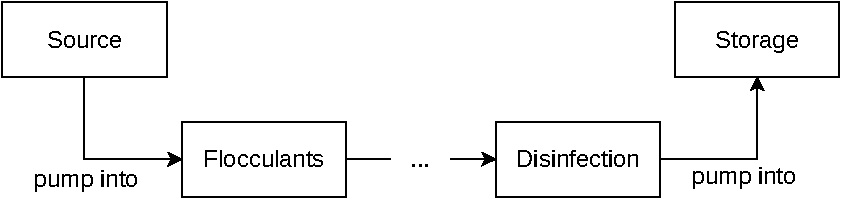
\includegraphics[width=12cm]{img/ch04/Testbed-Chain.pdf}
    \captionof{figure}{Chaining of the water treatment units, originating from a water source and eventually leading to a storage at the end of the processing pipeline.} %TODO: Describe
    \label{fig:testbed-chain}
\end{figure}
These units were then \enquote{chained} up (shown in figure \ref{fig:testbed-chain}) in the order in which they were presented in the scenario by specifying their direct predecessor and successor units: potentially contaminated water would be pumped out of the \emph{source}, processed by a series of stations and eventually flushed into the \emph{storage}. The \emph{source} was an instance of the \enquote{SourceUnit} that featured a throughput calculated by a sine-wave function that used the elapsed time since program startup as input parameter. Also, in order to keep the program running infinitely without either the \emph{source} \enquote{running dry} due to its input tank emptying or the \emph{storage} overfilling, the \emph{storage's} output was programmed to feed back into the \emph{source's} input tank (as can be seen in figure \ref{fig:mqtt-data}). While this was not a realistic approach, it kept the program's design simple and allowed for continuous testing and did not impact the \ac{MQTT} communication.

\begin{figure}[h]
    \centering
    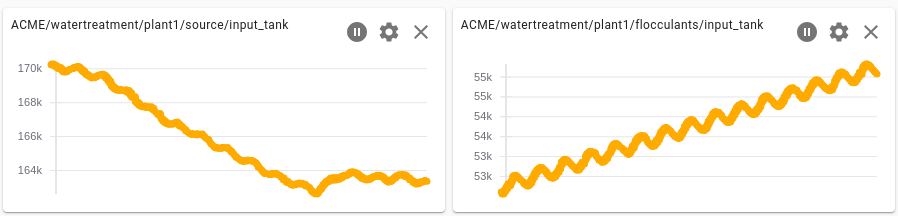
\includegraphics[width=14cm]{img/ch04/watertreatment-mqtt-short.png}
    \captionof{figure}{Screenshot of the application \enquote{MQTT Explorer} that was used to inspect and visualize the state of the water treatment plant. The left graph shows how the \emph{source's} input tank steadily emptied until it was filled by the \emph{storage's} output tank. The right graph shows how the \emph{flocculant} unit's input tank slowly filled up.} %TODO: Describe
    \label{fig:mqtt-data}
\end{figure}

\subsection{Implementation}
\emph{TBD:}  %TODO: Write out
\begin{itemize}
    \item \emph{technology: typescript}
    \item \emph{sprints: two sprints, started with communication (http + ws + mqtt)}
    \item \emph{failed: high-level API, callback-hell (debugging/tracing), missing typescript typings, very tight coupling}
\end{itemize}

\subsection{Insights Gained}
The following insights were gained through the prototypical implementation. Some resulted in questions relevant for the expert interviews that were to be held:
\begin{itemize}
    \item Due to the \ac{MTU}, large messages are broken into chunks that are transferred sequentially. This requires the proxy to work on streams of incoming data and reassemble messages from said chunks. % TODO: Also, stateful + buffers per connection
    \item Support of multiple clients is non-trivial as communication between clients and servers is not necessarily connection-oriented (e.g. \ac{HTTP}).\\
          \emph{Q: Do penetration testers need to test multiple devices at the same time?}
    \item Increasing the size of the payload of a messages can result in the payload being split upon multiple messages (e.g. \ac{WS}).\\
          \emph{Q: Do penetration testers require exact control over the implementation of protocols?}
    \item Manipulating messages, on the fly via scripting or by hand using third-party integrations (e.g. to \emph{Burp Suite}), can introduce latency to the communication. \emph{Q: Are there strict timing requirements during penetration tests?}
    \item Many libraries offer high-level functions to the programmer while avoiding exposure of low-level functionalities like crafting or parsing messages.
\end{itemize}


\section{Interviewing Experts for Insights}
\label{sec:interviews}
Interviews may be an efficient way to get an expert’s opinion on something they are proficient in. Thus, expert interviews were conducted to let security researchers give insight into their everyday work and the challenges they face when working with \ac{IoT} and \ac{IIoT} applications. The information and insights gathered in these interviews were then used to model a persona, various work scenarios and use-cases that as a whole aim to represent their work.

\subsection{Interview Guideline}
An interview guideline (shown in \emph{TBD}) %TODO: Reference appended interviews + guideline
was created to keep focus on key points during interviews so that interviewees would not stray too far from the relevant points. The guideline also served as a checklist so the interviewer could make sure that all questions and points that should be covered  initially, were in fact covered by the end of the interviews. It was composed of three sections:

\paragraph{1. Experiences with IoT} The answers to these questions would give insights into what kind of applications the security researchers had worked on in the past. Answers to question \emph{1.1.} were of particular interest as they might represent what technologies were being examined by security researchers and may be popular in today’s applications.
\paragraph{2. Processes in Everyday Life} This section aimed to cover questions about the processes and tasks security researchers perform during penetration tests of IoT applications in their everyday life. Ideally, answers to those questions would show the approaches taken and challenges faced during their work, uncovering potential needs and underlying motivation.
\paragraph{3. The Future of IoT} This section had security researchers assess what the future of IoT may be like from their point of view. This required the interviewees to make a critical assessment of the status quo.


\subsection{Conducting Interviews}
Interviews were conducted with six %Patrick, Cédric, Théo, Oliver, Pierre, Jonah
\emph{NVISO} employees that all had worked on security assignments on \ac{IoT} or \ac{IIoT} applications in the past. There is considerable variety in
\begin{itemize}
    \item the experience they had in working on security assignments in general: all interviewees had a strong background in cyber security that reached back multiple years except one who was a working student at \emph{NVISO Labs}.
    \item and the experience they had in working on \ac{IoT}/\ac{IIoT} applications: two interviewees worked on assessing \ac{IoT}/\ac{IIoT} applications only occasionally, one was part of a car manufacturer's automotive security team in the past and three were part of \emph{NVISO Labs} and worked with smart devices on a regular basis.
          % Position? CEO vs. Consultant vs. Working student
          % 
\end{itemize}
The duration of the interviews varied from 45 minutes to two hours depending on the amount and level of detail of information provided by the interviewees and the number of times that the interviewer had to ask further questions.

\emph{TBD:} %TODO: Write out
\begin{itemize}
    \item \emph{Summary of the interviews}
    \item \emph{conclusions drawn}
    \item \emph{personas and user stories -> new requirements!}
\end{itemize}

\section{Analysis of Existing Software}
\paragraph{Wireshark} more than 3,400,000 lines of C code\footnote{This number was returned by the \emph{cloc} utility run on commit \emph{3a8111e1c2adcdc0603993c6ed5d20a40f162125} from Aug. 4th 2020 of Wireshark's Github mirror.}\emph{TBD}
\paragraph{MITMf} \emph{TBD}
\paragraph{Ettercap} \emph{TBD}
\paragraph{bettercap} \emph{TBD}
\paragraph{mitmproxy} \emph{TBD}
\paragraph{mProxy} \emph{TBD}
\paragraph{IOXY} \emph{TBD}
\paragraph{scapy} \emph{TBD}

\emph{TBD; planned: paragraph about each program including a general description, uses, capabilities and usefulness} %TODO: Write out
\label{sec:analysis-existing-software}
\begin{table}[h]
    \centering
    \begin{tabular}{r|c|c|c|c|c|c}
        \toprule
        \thead{$Name$} & \thead{$Latest$                                                                                                    \\$Release$} & \thead{$Implemented$\\$in$} & \thead{$Supported$\\$Protocols$} & \thead{$R$} & \thead{$W$} & \thead{$D$}\\
        \midrule
        Wireshark      & 2020-07-01        & C      & Various    & \cellcolor{green!25}F  & \cellcolor{red!25}N    & \cellcolor{red!25}N    \\
        \midrule
        MITMf          & 2015-08-28        & Python & Various    & ?                      & \cellcolor{green!25}F  & \cellcolor{green!25}F  \\ %https://github.com/byt3bl33d3r/MITMf
        \midrule
        Ettercap       & 2019-07-01        & C      & Various    & \cellcolor{green!25}F  & \cellcolor{green!25}F  & \cellcolor{green!25}F  \\
        \midrule
        bettercap      & 2020-03-13        & Go     & Various    & \cellcolor{green!25}F  & \cellcolor{green!25}F  & \cellcolor{green!25}F  \\
        \midrule
        mitmproxy      & 2020-03-13        & Python & HTTP/S, WS & \cellcolor{orange!25}P & \cellcolor{orange!25}P & \cellcolor{orange!25}P \\ %https://github.com/mitmproxy/mitmproxy
        \midrule
        mProxy         & Pre-Releases only & Go     & MQTT       & ?                      & \cellcolor{green!25}F  & -                      \\ %https://github.com/mainflux/mproxy
        \midrule
        IOXY           & Source only       & Go     & MQTT       & \cellcolor{green!25}F  & \cellcolor{green!25}F  & \cellcolor{green!25}F  \\ %https://github.com/mainflux/mproxy
        \bottomrule
    \end{tabular}
    \caption[Comparison of existing software]{Comparison of existing software where $R$, $W$ and $D$ describe read, write and deletion capabilities, respectively. $F$, $N$ and $P$ indicate full, no or partial functionality, respectively.}
    \label{table:comparison-existing-software}
\end{table}